\documentclass[9pt]{article}
\usepackage[utf8]{inputenc}
\usepackage{geometry}
\geometry{letterpaper, margin=0.25in}
\usepackage{graphicx} 
\usepackage{multicol}
\usepackage{parskip}
\usepackage{booktabs}
\usepackage{array} 
\usepackage{paralist} 
\usepackage{verbatim}
\usepackage{sectsty}
\usepackage[shortlabels]{enumitem}

\usepackage{amsmath}
\usepackage{amssymb}
\usepackage{mathtools}
\usepackage{empheq}
\usepackage{xcolor}
\usepackage{bbm}
\usepackage{tikz}
\usepackage{pgfplots}
\usepackage{tikz-cd}
\usepackage{circuitikz}
\usepackage{multirow}
\pgfplotsset{compat=1.18}
\usetikzlibrary{intersections, decorations.markings}
\tikzset{
    marking along/.style n args={2}{
        decoration={
                markings, 
                mark=at position #1 with {\arrow{#2}}
        },
        postaction={decorate}
        },
    marking along/.default={0.5}{>}
    wavy/.style={
        decorate,decoration={coil,aspect=0}
     },
    two marks/.style n args={1}{
        decoration={
            markings,
            mark=at position 0.25 with {\arrow{#1}},
            mark=at position 0.75 with {\arrow{#1}}
         },
         postaction={decorate}
    }
    two marks/.default={>}
}

\colorlet{mygreen}{green!50!teal}
\colorlet{darkblue}{blue!60!black}

\newcommand{\ans}[1]{\boxed{\text{#1}}}
\newcommand{\vecs}[1]{\langle #1\rangle}
\renewcommand{\hat}[1]{\widehat{#1}}

\renewcommand{\P}{\mathbb{P}}
\newcommand{\R}{\mathbb{R}}
\newcommand{\E}{\mathbb{E}}
\newcommand{\Z}{\mathbb{Z}}
\newcommand{\N}{\mathbb{N}}
\newcommand{\Q}{\mathbb{Q}}
\newcommand{\C}{\mathbb{C}}

\newcommand{\ind}{\mathbbm{1}}
\newcommand{\qed}{\quad \blacksquare}

\newcommand{\brak}[1]{\left\langle #1 \right\rangle}
\newcommand{\bra}[1]{\left\langle #1 \right\vert}
\newcommand{\ket}[1]{\left\vert #1 \right\rangle}

\newcommand{\abs}[1]{\left\vert #1 \right\vert}
\newcommand{\mfX}{\mathfrak{X}}
\newcommand{\ep}{\varepsilon}

\newcommand{\Ec}{\mathcal{E}}
\newcommand{\Nc}{\mathcal{N}}
\newcommand{\A}{\mathcal{A}}
\newcommand{\F}{\mathcal{F}}
\newcommand{\Cc}{\mathcal{C}}
\newcommand{\B}{\mathcal{B}}
\newcommand{\M}{\mathcal{M}}
\newcommand{\X}{\chi}
\renewcommand{\L}{\mathcal{L}}

\newcommand{\sub}{\subseteq}
\newcommand{\st}{\text{ s.t. }}
\newcommand{\card}{\text{card }}
\renewcommand{\div}{\vspace*{10pt}\hrule\vspace*{10pt}}
\newcommand{\surj}{\twoheadrightarrow}
\newcommand{\inj}{\hookrightarrow}
\newcommand{\biject}{\hookrightarrow \hspace{-8pt} \rightarrow}
\renewcommand{\bar}[1]{\overline{#1}}
\newcommand{\overcirc}[1]{\overset{\circ}{#1}}
\newcommand{\diam}{\text{diam }}
\newcommand{\iid}{\overset{	ext{iid}}{\sim}}

\renewcommand{\Re}{\text{Re}\,}
\renewcommand{\Im}{\text{Im}\,}
\newcommand{\Var}{\text{Var}\,}
\newcommand{\Cov}{\text{Cov}\,}

\DeclareMathOperator*{\argmax}{\arg\max}
\DeclareMathOperator*{\argmin}{\arg\min}

\newcommand{\sign}{\text{sign}\,}

\newcommand*{\tbf}[1]{\ifmmode\mathbf{#1}\else\textbf{#1}\fi}

\usepackage{tcolorbox}
\tcbuselibrary{breakable, skins}
\tcbset{enhanced}
\newenvironment*{tbox}[2][gray]{
    \begin{tcolorbox}[
        parbox=false,
        colback=#1!5!white,
        colframe=#1!75!black,
        breakable,
        title={#2}
    ]}
    {\end{tcolorbox}}

\newenvironment*{exercise}[1][red]{
    \begin{tcolorbox}[
        parbox=false,
        colback=#1!5!white,
        colframe=#1!75!black,
        breakable
    ]}
    {\end{tcolorbox}}

\newenvironment*{proof}[1][blue]{
\begin{tcolorbox}[
    parbox=false,
    colback=#1!5!white,
    colframe=#1!75!black,
    breakable
]}
{\end{tcolorbox}}
\newenvironment*{proposition}[1][gray]{
    \begin{tcolorbox}[
        parbox=false,
        colback=#1!5!white,
        colframe=#1!75!black,
        breakable
    ]}
    {\end{tcolorbox}}


\begin{document}
\begin{multicols}{3}

\tbf{Linear system:} $L[au + bv] = aL[u] + bL[v], \quad a, b \in \R$

\tbf{LTI:} $y(t) = L[x(t)] \implies y(t - t_0) = L{x(t - t_0)}$

\tbf{Delta function:}
\begin{enumerate}
    \item $\int \delta(t)\; dt = 1$
    \item $\delta(t) = 0$ for $t \neq 0$
    \item $\int f(t) \delta(t - t_0)\; dt = f(t_0)$ (sifting)
\end{enumerate}

\tbf{Impulse response:} the output of an LTI system when the input is $\delta(t)$

\tbf{Transfer function:} $H(f) = \F(h(t))$ where $h(t)$ is the impulse response of the system.
\[y(t) = (x * h)(t) = \int_{-\infty}^\infty x(\tau) h(t - \tau) \; d\tau\]
(in fact, in the frequency domain, this operation is defined by $Y(f) = X(f) H(f)$)

\tbf{Fourier Transform:} 
\[\F[x(t)] = \int x(t)e^{-j\; 2\pi ft} \; dt = X(f)\]

\tbf{Inverse Fourier:} 
\[\F^{-1}[X(f)] = \int X(f) e^{j \; 2\pi ft} \; df = x(t)\]

\emph{Standard Fourier pairs:}
\begin{enumerate}
    \item $\F[\delta(t)] = 1$
    \item $\F[e^{-j\; 2\pi f_0 t}] = \delta(f + f_0)$
    \item $\F[\delta(t- t_0)] = e^{-j\; 2\pi f t_0}$
    \item $X(f - f_0) = x(t) e^{j\; 2\pi f_0 t}$
    \item $\F[\cos 2\pi f_0 t] = \frac{1}{2}[\delta(f + f_0) + \delta(f - f_0)]$
    \item $\F[\sin 2\pi f_0 t] = \frac{1}{2j}[\delta(f + f_0) - \delta(f - f_0)]$
    \item $\F[\ind_{x\in [-T/2, T/2]}] = \text{sinc}(2\pi Tf)$
\end{enumerate}

\emph{Fourier Properties:}
\begin{enumerate}
    \item $\F[x(t - t_0)] = e^{-j\; 2\pi f t_0} X(f)$
    \item $\F[x(at)] = \frac{1}{\abs a}X(f/a)$
    \item $\F[x'(t)] = X(f) \cdot j\; 2\pi f$
    \item $\F[\int_{-\infty}^t x(u)\; du] = \frac{X(f)}{j\; 2\pi f} + \frac{X(0)}{2} \delta(f)$
    \item $\int_{-\infty}^{\infty} \abs{x(t)}^2 = \int_{-\infty}^{\infty} \abs{X(f)}^2$ (Parseval's)
    \item $\F[x(-t)] = X(-f)$
    \item $\F[X(t)] = x(-f)$  
\end{enumerate}

\emph{Useful tricks:}
\begin{enumerate}
    \item $\abs{X(f)}^2 = X(f) X^*(f) = X(f) X(-f)$
    \item $\cos(2\pi f t) = (e^{j\; 2\pi f t} + e^{-j\; 2\pi f t})/2$
    \item $\sin(2\pi f t) = (e^{j\; 2\pi f t} - e^{-j\; 2\pi f t})/2j$
    \item Fourier of odd function is purely imaginary, Fourier of even function is purely real.
    \item $\delta$ is an even function: $\delta(-t) = \delta(t)$
    \item $\sin(x + y) = \sin x \cos y + \cos x \sin y$
    \item $\cos(x + y) = \cos x \cos y - \sin x \sin y$
    \item $\sin^2 x = (1 - \cos 2 x)/2$
    \item $\cos^2 x = (1 + \cos 2x)/ 2$
    \item $\cos \theta(t) = \sum_{m=0}^{\infty} \frac{(\theta(t))^{2m}}{(2m)!}$
    \item $\sin \theta(t) = \sum_{m=0}^{\infty} (-1)^m \frac{(\theta(t))^{2m+1}}{(2m + 1)!}$
    \item $\F[x(t)y(t)] = X(f) * Y(f)$
\end{enumerate}

\emph{Baseband:} unmodulated signal (i.e. the message signal).

\emph{Passband:} modulated signal (i.e. the transmitted signal).

\emph{AM Coherent modulation:} $r(t) = m(t) \cos 2\pi f_c t$, demodulate with $\cos 2\pi f_c t$ and LPF to recover $m(t)/2$.

\emph{AM Large carrier:} $r(t) = (m(t) + A) \cos 2\pi f_c t$ ($A \gg m(t)$), demodulate with an envelope detector, LPF, and HPF to recover $m(t)$.

\emph{AM Single sideband:} $r(t) = m(t) \cos 2\pi f_c t$ with an LPF applied to $m(t)$ before modulation (takes advantage of symmetry from $M(-f) = M^*(f)$ to use half the bandwidth), demodulate with $\cos 2\pi f_c t$ and LPF to recover $m(t)/2$.

\emph{Frequency modulation:} $r(t) = \sin (2\pi f_c t + \beta \int_{-\infty}^t m(\tau)\; d\tau)$, demodulate by differentiating, envelope detecting, and HPF to recover $\beta m(t)$.

\emph{Phase modulation:} $r(t) = \sin (2\pi f_c t + \beta m(t))$ (filter and integrate)

\emph{Carson's Rule:} $\Delta = (\kappa + 1)B$ where $\Delta$ is the single-sided FM bandwidth, $\kappa$ is the modulation index, and $B$ is the bandwidth of the message signal. 

\div 

\tbf{Sampling:} 
\begin{align*}
    \hat m(t) &= \sum_k m(Tk) \delta(t - Tk) \star \frac{\sin(\pi t / T)}{\pi t}\\
    &= \sum_k m(Tk) \frac{\sin(\pi(t - Tk)/T)}{\pi(t - Tk)/T}
\end{align*}
corresponding to adding copies of the spectrum at $[k/T - B, k/T+B]$ for $k \in \Z$ via delta functions and then low pass filtering. 

\tbf{Low pass filter:} 
\begin{align*}
    H(f) &= u(f + B) - u(f - B)\\ 
    h(t) &= \F^{-1}[H(f)] = \int_{-B}^B e^{-j\; 2\pi ft}\; df\\ 
    &= \frac{e^{-j\; 2\pi Bt} - e^{j\; 2\pi Bt}}{-j\; 2\pi t}\\ 
    & = \frac{\sin(2\pi Bt)}{\pi t} = \frac{\sin(\pi t/T)}{\pi t}
\end{align*}

\tbf{Nyquist Criterion:} $T < 1/2B$ (i.e. sample at rate $T$ to avoid the sampled spectra from overlapping)
\begin{itemize}
    \item $m(t) \cos 2\pi t$ has bandwidth $B = 1$ 
    \item $m(t) \cos 2\pi f_ct$ has frequency in $[f_c - B, f_c + B]$ so we need $T < 1/2(f_c + B)$
\end{itemize}

\tbf{Expected quantization error:} 
\[\int f_M(m) (m - Q(m))^2\; dm\]

\tbf{Leibniz's Rule:} 
\begin{align*}
    \frac{d}{dx} &\int_{a(x)}^{b(x)} f(x, y)\; dy =\\ 
    &f(x, b(x)) \cdot \frac{db}{dx}
     - f(x, a(x)) \cdot \frac{da}{dx} \\ 
    &+ \int_{a(x)}^{b(x)} \frac{\partial f}{\partial x}\; dy
\end{align*}


\tbf{Lloyd max optimal quantizer:} 
\begin{enumerate}
    \item $x_i = \frac{1}{2}(q_{i+1} + q_i)$
    \item $q_i = \E[M \; | \; m \in (x_{i-1}, x_i)]$
\end{enumerate}
(should be symmetric and have $N = 2^b$ quantization levels for $b$ bits)
\begin{center}
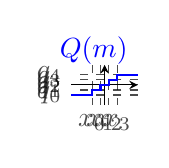
\begin{tikzpicture}
\begin{axis}[
    width=0.2\textwidth,
    axis lines=middle,
    no markers,
    xtick=\empty,
    ytick=\empty,
    clip=false,
    xlabel={},
    ylabel={},
    domain=-2:2,
    ymin=-2, ymax=2,
    xmin= -2, xmax=2,
    view = {0}{90}
]
    \draw[dashed, opacity=0.7] (2, 1) -- (-2, 1) node[left] {$q_4$};
    \draw[dashed, opacity=0.7] (2, 0.5) -- (-2, 0.5) node[left] {$q_3$};
    \draw[dashed, opacity=0.7] (2, 0) -- (-2, 0) node[left] {$q_2$};
    \draw[dashed, opacity=0.7] (2, -0.5) -- (-2, -0.5) node[left] {$q_1$};
    \draw[dashed, opacity=0.7] (2, -1) -- (-2, -1) node[left] {$q_0$};

    \draw[dashed, opacity=0.7] (-0.75, 2) -- (-0.75, -2) node[below] {$x_0$};
    \draw[dashed, opacity=0.7] (-0.25, 2) -- (-0.25, -2) node[below] {$x_1$};
    \draw[dashed, opacity=0.7] (0.25, 2) -- (0.25, -2) node[below] {$x_2$};
    \draw[dashed, opacity=0.7] (0.75, 2) -- (0.75, -2) node[below] {$x_3$};

    \addplot[thick, blue] coordinates { (-2, -1) (-0.75, -1) (-0.75, -0.5) (-0.25, -0.5) (-0.25, 0) (0.25, 0) (0.25, 0.5) (0.75, 0.5) (0.75, 1) (2, 1)} node[above left] {$Q(m)$};
\end{axis}
\end{tikzpicture}
\end{center}

\tbf{Convexity:} $f(x_1, \dots, x_n)$ convex iff $\forall x_1, x_2 \in \R^n$, $\lambda \in [0, 1]$, 
\[f(\lambda x_1 + (1- \lambda)x_2) \leq \lambda f(x_1) + (1 - \lambda) f(x_2)\]

\tbf{Hessian:} 
\[H_f(x) = \begin{bmatrix}
\frac{\partial^2 f}{\partial x_1^2} & \cdots & \frac{\partial^2 f}{\partial x_1 \partial x_n}\\
\vdots & \ddots & \vdots\\
\frac{\partial^2 f}{\partial x_n \partial x_1} & \cdots & \frac{\partial^2 f}{\partial x_n^2}\end{bmatrix}\]

$f$ is convex iff $H_f(x)$ is positive semidefinite for all $x$: $x^{\top} H_f(x) x \geq 0$ (equivalently all eigenvalues of $H_f(x)$ are nonnegative for all $x$)

\tbf{PMF:} $f_X(x) = \P(X = x)$ with $\int f_X(x)\; dx = 1$ and $f_X(x) \geq 0$ for all $x$.

\tbf{CDF:} $F_X(x) = \P(X \leq x) = \int_{-\infty}^x f_X(t)\; dt$

\tbf{Expectation:} $\E[X] = \int x f_X(x)\; dx$ 

\tbf{Variance:} $\Var[X] = \E[(X - \E[X])^2] = \E[X^2] - (\E[X])^2 = \sigma_X^2$

\tbf{Joint random variables:} 
\begin{enumerate}
    \item $\int \int f_{X, Y}(x, y) \; dx\, dy = 1$
    \item $f_{X, Y}(x, y) \geq 0$ 
\end{enumerate}

\tbf{Marginals:} 
\begin{align*}
    f_X(x) &= \int f_{X, Y}(x, y)\; dy\\ 
    f_Y(y) &= \int f_{X, Y}(x, y)\; dx
\end{align*}


\tbf{Marginal Expectation:}
\[\E[X] = \int \int x f_{X, Y}(x, y)\; dx \, dy\]

\tbf{Conditional probability:}
\[f_{X|Y}(x| y) = \frac{f_{X, Y}(x, y)}{f_Y(y)} \]

\tbf{Bayes:} $f_{X, Y}(x, y) = f_{X|Y}(x|y) f_Y(y) = f_{Y|X}(y|x) f_X(x)$

\tbf{Independece:} $f_{X|Y}(x|y) = f_X(x)$ 

\tbf{Correlation:} 
\[\E[X Y] = \int \int x y f_{X, Y}(x, y)\; dx\, dy\]

\tbf{Covariance:} $\Cov[X, Y] = \E[(X - \E[X])(Y - \E[Y])] = \int \int (X - \bar X)(Y - \bar Y)f_{X, Y}(x, y)\; dx\, dy$

\emph{Trick:} If $\E[X] = 0$ and $\Var[X] = \E[X^2] = 0$, then $X = \E[X] = 0 $ a.e. 

$X, Y$ independent implies 
\begin{enumerate}
    \item $f_{X, Y}(x, y) = f_X(x) f_Y(y)$
    \item $\E[X Y] = \E[X] \E[Y]$
    \item $\Cov[X, Y] = 0$
\end{enumerate}

\tbf{Gaussian:} 
\begin{align*}
    f_X(x) &= \frac{1}{\sqrt{2\pi \sigma^2}} e^{-(x - \mu)^2/2\sigma^2}\\ 
    f_X(x_{1:N}) &= \frac{\exp\left(-\frac{1}{2} (x - \mu)^{\top} K^{-1} (x - \mu)\right)}{(2\pi)^{N/2} \sqrt{\det K}}
\end{align*}
\begin{align*}
     K &= \E[(x - \mu)(x - \mu)^{\top}]\\ 
    &= \begin{pmatrix}
        \sigma_1^2 & \Cov[X_1, X_2] & \dots \\ 
        \Cov[X_2, X_1] & \sigma_2^2 & \dots \\
        \vdots & \vdots & \ddots\\
    \end{pmatrix}
\end{align*}


For $X, Y$ jointly gaussian, $\Cov(X, Y) = 0 \implies X, Y$ independent. Further, any linear combination of jointly gaussian random variables is also (jointly) gaussian.

\tbf{Adding random variables:} \begin{align*}
    f_{X + Y}(z) &= \int f_X(x) f_Y(z - x)\; dx\\ 
    &= (f_X \star f_Y)(z)
\end{align*}
For $X, Y$ independent gaussian, $X + Y$ is gaussian with mean $\mu_X + \mu_Y$ and variance $\sigma_X^2 + \sigma_Y^2$.

$X, Y$ independent implies 
\begin{enumerate}
    \item $f_{X, Y}(x, y) = f_X(x) f_Y(y)$
    \item $\E[X Y] = \E[X] \E[Y]$
    \item $\Cov[X, Y] = 0$
\end{enumerate}

\tbf{Random process:} $X: \omega \mapsto f(t, \omega)$ (random variable for each fixed $t$, random function for each fixed $\omega$)

\tbf{Stationary Gaussian process:} 
\begin{enumerate}
    \item Mean: $\E[X(t)] = 0$
    \item Covariance: $\E[X(s) X(t)] = K(s - t)$ for some function $L$ (i.e. depends only on the time difference)
\end{enumerate}

The covariance function and covariance matrix are related by 
\begin{align*}
    K &= \E\begin{bmatrix}
        \begin{pmatrix}
            X(t_1)\\ 
            X(t_2)
        \end{pmatrix} \begin{pmatrix}
            X(t_1) & X(t_2)
        \end{pmatrix}
    \end{bmatrix}\\ 
    &= \begin{pmatrix}
        K(0) & K(t_1 - t_2)\\ 
        K(t_2 - t_1) & K(0)
    \end{pmatrix}
\end{align*}
with $K(t_1 - t_2) = K(t_2 - t_1)$ 

\tbf{White Gaussian Process:} $K(s - t) = N_0 \delta(s - t)$

\tbf{Spectral Density:} $S_X(f) = \F[K(\tau)]$ (Fourier transform of the covariance function)

\tbf{Autocorrelation:} $R_{\tau} = \E[X(t) X(t + \tau)]$ (same as covariance for zero-mean processes)

\tbf{Gaussian LTIs:} Let $X$ be stationary white gaussian and $h(t)$ be the impulse response of an LTI system. Then for $Y = h \star X$,
\begin{align*}
    & \E[Y] = \int h(t - \tau) \E[X(\tau)]\; d\tau = 0\\
    & K_Y(\tau) = \E[Y(t) Y(t + \tau)]\\ 
    &= \E\left[\int \int X(\lambda) X(\sigma) h(t - \lambda) h(t + \tau - \sigma)\; d\sigma d\lambda \right]\\ 
    &= \E\left[\int \int K_X(\lambda - \sigma) h(t - \lambda) h(t + \tau - \sigma) \; d\lambda \, d\sigma\right]\\ 
    &= N_0 \int h(t - \sigma) h(t + \tau - \sigma)\; d\sigma 
\end{align*}

\tbf{Cauchy-Schwarz:} 
\[\left(\int x(t) y(t)\right)^2 \leq \int \abs{x(t)}^2\; dt \cdot \int \abs{y(t)}^2\; dt\]

\tbf{Energy:} $\Ec_x = \int \abs{x(t)}^2\; dt$

\tbf{Matched filter:} $h(t) = x(T - t)$ maximizes the SNR ($\abs{b} \Ec_x/N_0$) at time $T$ for a signal $x(t)$ corrupted by white gaussian noise.

Equivalent to maximizing the correlation $\int (bx(t) + w(t)) x(t)\; dt = b\int_0^T \abs{x(t)}^2\; dt + \int_0^T w(t) x(t)\; dt$ 

\tbf{Probability of error:} 
\begin{align*}
    P_e &= \P(\hat b = 1 | b= -1)(1 - p)\\ 
    &\qquad + \P(\hat b = -1 | b=1)p\\ 
    &= (1 - p) \int_D f_{Y|b=-1}(y | b=-1)\; dy\\ 
    &\qquad + p \int_{D^c} f_{Y|b=1}(y | b=1)\; dy
\end{align*}
(precisely the area under the overlapping tails of the two distributions)

\tbf{Decision Rule:}
\[\begin{cases}
    \frac{p f_{R | b=1}}{(1 - p) f_{R| b=-1}} > 1 \implies \hat b = 1\\
    \frac{p f_{R | b=1}}{(1 - p) f_{R| b=-1}} < 1 \implies \hat b = -1
\end{cases}\]
\end{multicols}

\end{document}